\documentclass[12pt]{article}

%-------------PACKAGES------------- 
\usepackage[margin=1in]{geometry} 
\usepackage{amsmath,amsthm,amssymb}
\usepackage{pgfplots}
\usepackage{float}
\usepackage{braket}
\usepackage{titling}
\usepackage{tikz}
\usepackage{mwe}
\usepackage{booktabs}
\usepackage{pifont}
\usepackage{array,graphicx}
\usepackage{tabularx,colortbl}
\usepackage{mathtools}
\usepackage{listings}
\usepackage{color}
\usepackage{caption}
\usepackage{subcaption}
\usepackage{algorithm,algpseudocode}
\usetikzlibrary{shapes,arrows,chains}
\usetikzlibrary[calc]

%-------------FORMATTING-------------
\setlength{\droptitle}{-8.5em} 
\setlength{\parindent}{0pt}
\def\LW{\dimexpr.25\linewidth-.5em} 
\tikzstyle{line} = [draw, -latex']
 
%--------------COMMANDS--------------
\newcommand{\N}{\mathbb{N}}
\newcommand{\Z}{\mathbb{Z}}
\newcommand{\R}{\mathbb{R}}
\newcommand{\C}{\mathbb{C}}
%\renewcommand{\qedsymbol}{\filledbox}
\newcommand*\rot{\rotatebox{90}}
\newcommand*\OK{\ding{51}}

\DeclarePairedDelimiter \abs{\lvert}{\rvert}%
\DeclarePairedDelimiter \babs{\bigg\lvert}{\bigg\rvert}%
\DeclarePairedDelimiter \norm{\lVert}{\rVert}%

%------------ENVIRONMENTS------------- 
\newenvironment{theorem}[2][]{\begin{trivlist}
\item[{\bfseries #1}\hskip \labelsep {\bfseries #2.}]}{\end{trivlist}}
\newenvironment{lemma}[2][Lemma]{\begin{trivlist}
\item[\hskip \labelsep {\bfseries #1}\hskip \labelsep {\bfseries #2.}]}{\end{trivlist}}
\newenvironment{exercise}[2][Exercise]{\begin{trivlist}
\item[\hskip \labelsep {\bfseries #1}\hskip \labelsep {\bfseries #2.}]}{\end{trivlist}}
\newenvironment{reflection}[2][Reflection]{\begin{trivlist}
\item[\hskip \labelsep {\bfseries #1}\hskip \labelsep {\bfseries #2.}]}{\end{trivlist}}
\newenvironment{proposition}[2][Proposition]{\begin{trivlist}
\item[\hskip \labelsep {\bfseries #1}\hskip \labelsep {\bfseries #2.}]}{\end{trivlist}}
\newenvironment{corollary}[2][Corollary]{\begin{trivlist}
\item[\hskip \labelsep {\bfseries #1}\hskip \labelsep {\bfseries #2.}]}{\end{trivlist}}
\newenvironment{definition}[2][]{\begin{trivlist}
\item[{\bfseries #1}\hskip \labelsep {\bfseries #2.}]}{\end{trivlist}}
\theoremstyle{remark}
\newtheorem*{remark}{Remark}

%-------------CODE-STYLE------------
\definecolor{dkgreen}{rgb}{0,0.6,0}
\definecolor{gray}{rgb}{0.5,0.5,0.5}
\definecolor{mauve}{rgb}{0.58,0,0.82}
\lstset{frame=tb,
	language=C++,
	aboveskip=3mm,
	belowskip=3mm,
	showstringspaces=false,
	columns=flexible,
	basicstyle={\small\ttfamily},
	numbers=none,
	numberstyle=\tiny\color{gray},
	keywordstyle=\color{blue},
	commentstyle=\color{dkgreen},
	stringstyle=\color{mauve},
	breaklines=true,
	breakatwhitespace=true,
	tabsize=3
}

\tikzset{
	path image/.style={
		path picture={
			\node at (path picture bounding box.center) {
				\includegraphics[height=3cm]{example-image}};}},
	path tikzimage/.style={
		path picture={
			\node at (path picture bounding box.center)
			[circle, fill=blue!50, scale=2, text=yellow]{Bravo};}}
}
	
\lstset{
	morekeywords={end}
}

%------------------------------------ 
%---------START-OF-DOCUMENT----------
%------------------------------------
\begin{document}
 
\title{Homework 1 \\ CIS 5371: Cryptography} 
\author{David Miller \& Hannah McLaughlin}
\date{\vspace{-.5cm} January 25, 2018}

\maketitle

\textit{\textbf{Problem 1:} In class, we learned about the dating problem and the 5-card trick. Prove that the trick protects the privacy of Bob.} \\

Let a message $m$ in our message space $\mathcal{M}$ be a two-tuple \{Alice's decision, Bob's decision\} where 1 represents "yes" and 0 represents "no". To protect Bob's privacy we must show 
\begin{align}
	\underset{K \xleftarrow[]{\$} \mathcal{K}}{\text{Pr}}[\mathcal{E}_K(m_0) = c] = 
	\underset{K \xleftarrow[]{\$} \mathcal{K}}{\text{Pr}}[\mathcal{E}_K(m_1) = c]
\end{align}
where $m_0 = \{0,1\}$, $m_1 = \{0,0\}$, and $c$ is some ciphertext. This can be shown via the group table for cuts made by Alice and Bob. This is because a cut in the deck is simply a shift. If we let $p$ be the position where a cut is made then a cut maps Card$_i$ $\rightarrow$ Card$_{i - p \hspace{.05cm} \text{mod} \hspace{.05cm} 5}$ for $i = 0, ..., 4$. In fact the cut operation can be composed with another cut allowing us to represent the result from Alice's and Bob's cut in a group table. Letting $c_0(m_0)$ and $c_0(m_1)$ be the original ordering of cards before cuts, we can find the result after the two cuts with figure 1 where $c_n$ represents the shift Card$_i$ $\rightarrow$ Card$_{i - p \hspace{.05cm} \text{mod} \hspace{.05cm} 5}$. The result after applying $c_n$ is the ciphertext $c$.
\vspace{-.1 cm}
\begin{figure}[H]
\noindent\begin{minipage}{.35\linewidth}%
\begin{center}
	\vskip .1cm
	\begin{tabular}{|c||c|c|c|c|c|}
		\multicolumn{6}{c}{\hspace{.7 cm} Bob's Cut} \\
		\hline
		$\cdot$ & $\boldsymbol{c_0}$ & $\boldsymbol{c_1}$ & $\boldsymbol{c_2}$ & $\boldsymbol{c_3}$ & $\boldsymbol{c_4}$ \\ \hline \hline
		$\boldsymbol{c_0}$ & $c_0$ & $c_1$ & $c_2$ & $c_3$ & $c_4$ \\ \hline
		$\boldsymbol{c_1}$ & $c_1$ & $c_2$ & $c_3$ & $c_4$ & $c_0$ \\ \hline
		$\boldsymbol{c_2}$ & $c_2$ & $c_3$ & $c_4$ & $c_0$ & $c_1$ \\ \hline
		$\boldsymbol{c_3}$ & $c_3$ & $c_4$ & $c_0$ & $c_1$ & $c_2$ \\ \hline
		{\hspace{-.95cm} \rot{\rlap{Alice's Cut}}}
		$\hspace{0.4cm}\boldsymbol{c_4}$ & $c_4$ & $c_0$ & $c_1$ & $c_2$ & $c_3$ \\ \hline 
	\end{tabular}
	\vskip .5cm
\end{center}
\end{minipage}%
\begin{minipage}{.65\linewidth}
	\begin{tikzpicture}
		\node[] at (0,0) {$c_0(m_0)$:};
		\node[inner sep=0pt] (whitehead) at (1.25,0)
		{
\includegraphics[width=.075\textwidth]{heart.png}};
		\node[inner sep=0pt] (whitehead) at (2,0)
		{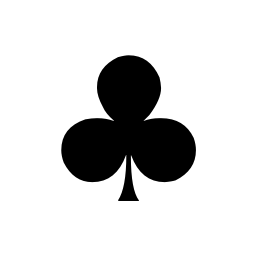
\includegraphics[width=.1\textwidth]{club.png}};
		\node[inner sep=0pt] (whitehead) at (2.75,0)
		{
\includegraphics[width=.075\textwidth]{heart.png}};
		\node[inner sep=0pt] (whitehead) at (3.5,0)
		{
\includegraphics[width=.075\textwidth]{heart.png}};
		\node[inner sep=0pt] (whitehead) at (4.25,0)
		{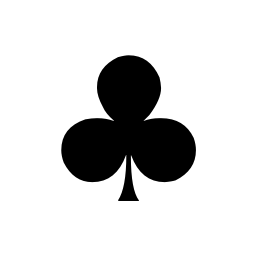
\includegraphics[width=.1\textwidth]{club.png}};
		
		\node[] at (0,-1) {$c_1(m_0)$:};
		\node[inner sep=0pt] (whitehead) at (1.25,-1)
		{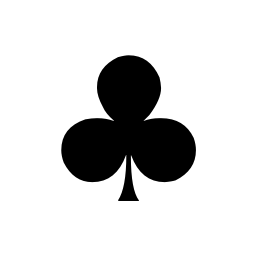
\includegraphics[width=.1\textwidth]{club.png}};
		\node[inner sep=0pt] (whitehead) at (2,-1)
		{
\includegraphics[width=.075\textwidth]{heart.png}};
		\node[inner sep=0pt] (whitehead) at (2.75,-1)
		{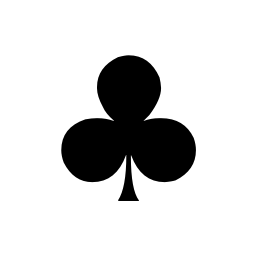
\includegraphics[width=.1\textwidth]{club.png}};
		\node[inner sep=0pt] (whitehead) at (3.5,-1)
		{
\includegraphics[width=.075\textwidth]{heart.png}};
		\node[inner sep=0pt] (whitehead) at (4.25,-1)
		{
\includegraphics[width=.075\textwidth]{heart.png}};
		
		\node[] at (0,-2) {$c_2(m_0)$:};
		\node[inner sep=0pt] (whitehead) at (1.25,-2)
		{
\includegraphics[width=.075\textwidth]{heart.png}};
		\node[inner sep=0pt] (whitehead) at (2,-2)
		{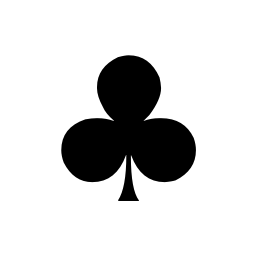
\includegraphics[width=.1\textwidth]{club.png}};
		\node[inner sep=0pt] (whitehead) at (2.75,-2)
		{
\includegraphics[width=.075\textwidth]{heart.png}};
		\node[inner sep=0pt] (whitehead) at (3.5,-2)
		{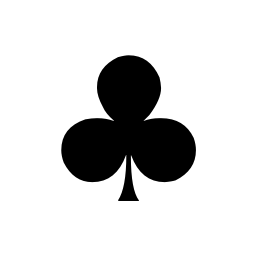
\includegraphics[width=.1\textwidth]{club.png}};
		\node[inner sep=0pt] (whitehead) at (4.25,-2)
		{
\includegraphics[width=.075\textwidth]{heart.png}};
		
		\node[] at (0,-3) {$c_3(m_0)$:};
		\node[inner sep=0pt] (whitehead) at (1.25,-3)
		{
\includegraphics[width=.075\textwidth]{heart.png}};
		\node[inner sep=0pt] (whitehead) at (2,-3)
		{
\includegraphics[width=.075\textwidth]{heart.png}};
		\node[inner sep=0pt] (whitehead) at (2.75,-3)
		{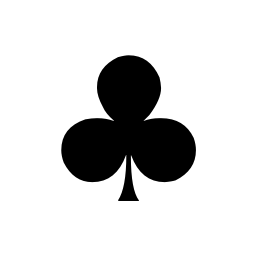
\includegraphics[width=.1\textwidth]{club.png}};
		\node[inner sep=0pt] (whitehead) at (3.5,-3)
		{
\includegraphics[width=.075\textwidth]{heart.png}};
		\node[inner sep=0pt] (whitehead) at (4.25,-3)
		{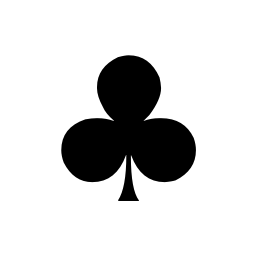
\includegraphics[width=.1\textwidth]{club.png}};
		
		\node[] at (0,-4) {$c_4(m_0)$:};
		\node[inner sep=0pt] (whitehead) at (1.25,-4)
		{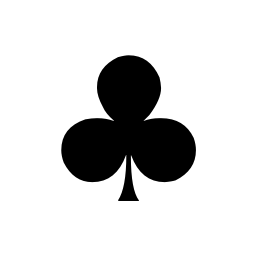
\includegraphics[width=.1\textwidth]{club.png}};
		\node[inner sep=0pt] (whitehead) at (2,-4)
		{
\includegraphics[width=.075\textwidth]{heart.png}};
		\node[inner sep=0pt] (whitehead) at (2.75,-4)
		{
\includegraphics[width=.075\textwidth]{heart.png}};
		\node[inner sep=0pt] (whitehead) at (3.5,-4)
		{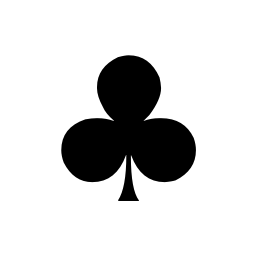
\includegraphics[width=.1\textwidth]{club.png}};
		\node[inner sep=0pt] (whitehead) at (4.25,-4)
		{
\includegraphics[width=.075\textwidth]{heart.png}};
		
		\node[] at (5.75,0) {$c_0(m_1)$:};
		\node[inner sep=0pt] (whitehead) at (7,0)
		{
\includegraphics[width=.075\textwidth]{heart.png}};
		\node[inner sep=0pt] (whitehead) at (7.75,0)
		{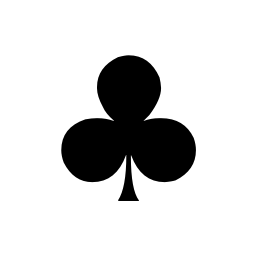
\includegraphics[width=.1\textwidth]{club.png}};
		\node[inner sep=0pt] (whitehead) at (8.5,0)
		{
\includegraphics[width=.075\textwidth]{heart.png}};
		\node[inner sep=0pt] (whitehead) at (9.25,0)
		{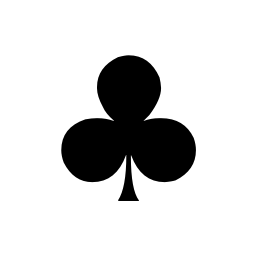
\includegraphics[width=.1\textwidth]{club.png}};
		\node[inner sep=0pt] (whitehead) at (10,0)
		{
\includegraphics[width=.075\textwidth]{heart.png}};
		
		\node[] at (5.75,-1) {$c_1(m_1)$:};
		\node[inner sep=0pt] (whitehead) at (7,-1)
		{
\includegraphics[width=.075\textwidth]{heart.png}};
		\node[inner sep=0pt] (whitehead) at (7.75,-1)
		{
\includegraphics[width=.075\textwidth]{heart.png}};
		\node[inner sep=0pt] (whitehead) at (8.5,-1)
		{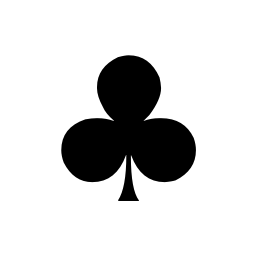
\includegraphics[width=.1\textwidth]{club.png}};
		\node[inner sep=0pt] (whitehead) at (9.25,-1)
		{
\includegraphics[width=.075\textwidth]{heart.png}};
		\node[inner sep=0pt] (whitehead) at (10,-1)
		{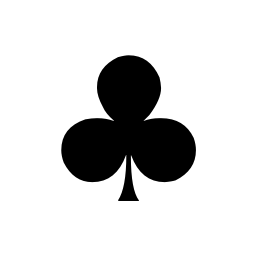
\includegraphics[width=.1\textwidth]{club.png}};
		
		\node[] at (5.75,-2) {$c_2(m_1)$:};
		\node[inner sep=0pt] (whitehead) at (7,-2)
		{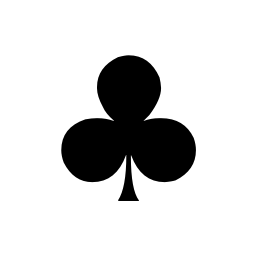
\includegraphics[width=.1\textwidth]{club.png}};
		\node[inner sep=0pt] (whitehead) at (7.75,-2)
		{
\includegraphics[width=.075\textwidth]{heart.png}};
		\node[inner sep=0pt] (whitehead) at (8.5,-2)
		{
\includegraphics[width=.075\textwidth]{heart.png}};
		\node[inner sep=0pt] (whitehead) at (9.25,-2)
		{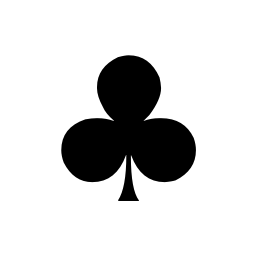
\includegraphics[width=.1\textwidth]{club.png}};
		\node[inner sep=0pt] (whitehead) at (10,-2)
		{
\includegraphics[width=.075\textwidth]{heart.png}};
		
		\node[] at (5.75,-3) {$c_3(m_1)$:};
		\node[inner sep=0pt] (whitehead) at (7,-3)
		{
\includegraphics[width=.075\textwidth]{heart.png}};
		\node[inner sep=0pt] (whitehead) at (7.75,-3)
		{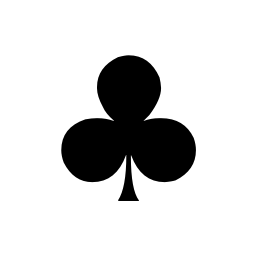
\includegraphics[width=.1\textwidth]{club.png}};
		\node[inner sep=0pt] (whitehead) at (8.5,-3)
		{
\includegraphics[width=.075\textwidth]{heart.png}};
		\node[inner sep=0pt] (whitehead) at (9.25,-3)
		{
\includegraphics[width=.075\textwidth]{heart.png}};
		\node[inner sep=0pt] (whitehead) at (10,-3)
		{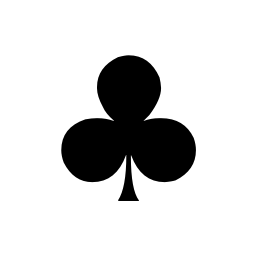
\includegraphics[width=.1\textwidth]{club.png}};
		
		\node[] at (5.75,-4) {$c_4(m_1)$:};
		\node[inner sep=0pt] (whitehead) at (7,-4)
		{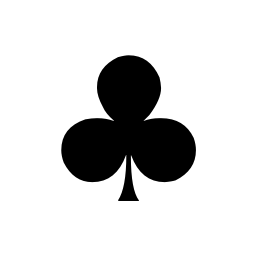
\includegraphics[width=.1\textwidth]{club.png}};
		\node[inner sep=0pt] (whitehead) at (7.75,-4)
		{
\includegraphics[width=.075\textwidth]{heart.png}};
		\node[inner sep=0pt] (whitehead) at (8.5,-4)
		{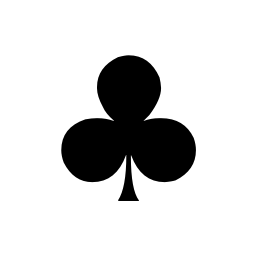
\includegraphics[width=.1\textwidth]{club.png}};
		\node[inner sep=0pt] (whitehead) at (9.25,-4)
		{
\includegraphics[width=.075\textwidth]{heart.png}};
		\node[inner sep=0pt] (whitehead) at (10,-4)
		{\includegraphics[width=.075\textwidth]{heart.png}};
	\end{tikzpicture}
\end{minipage}
\caption{Group table of shifts on $m_0$ and $m_1$ and their corresponding outcome.}
\end{figure}
Since we are considering Alice's viewpoint, we have a prescribed cut $c_m$ by Alice. Now Bob randomly picks $c_n$ for $n$ uniformly distributed over 0, \dots, 4. The composition $c_{m + n \hspace{.05cm} mod \hspace{.05cm} 5}$ will be a secret cyclic shift to Alice via Card$_i$ $\rightarrow$ Card$_{i - p \hspace{.05cm} \text{mod} \hspace{.05cm} 5}$. Since $c_0(m_1) = c_2(m_0)$ we get
\begin{align}
\underset{K \xleftarrow[]{\$} \mathcal{K}}{\text{Pr}}[\mathcal{E}_K(m_0) = c] = \frac{1}{5} =
\underset{K \xleftarrow[]{\$} \mathcal{K}}{\text{Pr}}[\mathcal{E}_K(m_1) = c]
\end{align}
from Alice's perspective and therefore the privacy of Bob is protected.
\qed

\newpage

\textit{\textbf{Problem 2:} Alice shuffles a deck of cards and deals it out to herself and Bob so that each gets half of the 52 cards. Alice now wishes to send a secret message $M$ to Bob by saying something aloud. Eavesdropper Eve is listening in hearing everything Alice says but can’t see the cards.} \\

\textit{\textbf{Part A:} Suppose Alice's message $M$ is a string of 48-bits, so the message space $M$ = \{0, 1\}$^{48}$. Describe how Alice can communicate $M$ to Bob to achieve perfect secrecy.} \\

Let $\mathcal{M}$ denote the message space of 48-bit strings, and $\mathcal{C}$ denote the ciphertext space. We have that $\abs{\mathcal{M}}$ = $2^{48}$ $<$ ${}_{52}C_{26}$ = $\abs{\mathcal{K}}$ and therefore $\abs{\mathcal{C}} = \abs{\mathcal{K}}$. Now define the encryption algorithm as 
\begin{align}
	& \mathcal{E}_K(m): \mathcal{M} \rightarrow \mathcal{C} \\
	& \mathcal{E}_K(m) = (m + k) \mod {}_{52}C_{26}
\end{align}
for $k \in \mathcal{K}, c \in \mathcal{C}$. Respectively, define the decryption algorithm as
\begin{align}
	& \mathcal{E}^{-1}_K(c): \mathcal{C} \rightarrow \mathcal{M} \\
	& \mathcal{E}^{-1}_K(c) = (c - k) \mod 2^{48}
\end{align}
for $k \in \mathcal{K}, c \in \mathcal{C}$. Both $\mathcal{E}_K, \mathcal{E}^{-1}_K$ are one-to-one functions and therefore deterministic. To prove perfect secrecy we must show (1). It will be shown from implication rather than directly. For $m \in \mathcal{M}, c \in \mathcal{C}$ we have 
\begin{align}
		& \underset{K \xleftarrow[]{\$} \mathcal{K}}{\text{Pr}}[\text{Alice says } c \hspace{0.05cm} \vert \hspace{0.05cm} M = m] =
		\underset{K \xleftarrow[]{\$} \mathcal{K}}{\text{Pr}}[\mathcal{E}_K(m) = c \text{ \hspace{.05cm}mod} {}_{52}C_{26}] =
		\\
		& \underset{K \xleftarrow[]{\$} \mathcal{K}}{\text{Pr}}[\mathcal{E}_K(m) = (m + (c - m)) \text{ \hspace{.05cm}mod} {}_{52}C_{26}]
		= \underset{K \xleftarrow[]{\$} \mathcal{K}}{\text{Pr}}[k = (c - m) \text{ \hspace{.05cm}mod} {}_{52}C_{26}] = \frac{1}{{}_{52}C_{26}}.
\end{align}
It follows from (7) and (8) that 
\begin{align}
	\underset{K \xleftarrow[]{\$} \mathcal{K}}{\text{Pr}}[\mathcal{E}_K(m_0) = c] = 
	\underset{K \xleftarrow[]{\$} \mathcal{K}}{\text{Pr}}[\mathcal{E}_K(m_1) = c]
\end{align}
for $m_0, m_1 \in \mathcal{M}, c \in \mathcal{C}$. It is important to note for (7) and (8) we used the fact that the key is sampled from a uniform distribution. \qed \\

\textit{\textbf{Part B:} Now suppose Alice's message $M$ is 49 bits, so the message space is $M$ = \{0, 1\}$^{49}$. Prove that there exists no protocol that allows Alice to communicate M to Bob to achieve perfect secrecy.} \\

Let $\mathcal{M}$ denote the message space of 49-bit strings. Now we have $\abs{\mathcal{K}} = {}_{52}C_{26} < 2^{49} = \abs{\mathcal{M}}$ and therefore $\abs{\mathcal{C}} = \abs{\mathcal{K}}$.  \\

\textit{Proof 1}: Since $\abs{\mathcal{K}} < \abs{\mathcal{M}}$ there exists $m_0, m_1 \in \mathcal{M}$ such that $\mathcal{E}_k(m_0) = \mathcal{E}_k(m_1) = c$ for some ciphertext $c \in \mathcal{C}$. Therefore 
\begin{align}
	& \underset{K \xleftarrow[]{\$} \mathcal{K}}{\text{Pr}}[\mathcal{E}_K(m_0) = c] =
	\underset{K \xleftarrow[]{\$} \mathcal{K}}{\text{Pr}}[\mathcal{E}_K(m_0) = \mathcal{E}_K(m_1)] = 
	\underset{K \xleftarrow[]{\$} \mathcal{K}}{\text{Pr}}[\mathcal{E}_K(\mathcal{E}_K^{-1}(c)) = \mathcal{E}_K(m_1)] \\
	& \underset{K \xleftarrow[]{\$} \mathcal{K}}{\text{Pr}}[\mathcal{E}_K(m_1) = \mathcal{E}_K(m_1)] = 1
\end{align}
We have arrived at the contradiction
\begin{align}
	\underset{K \xleftarrow[]{\$} \mathcal{K}}{\text{Pr}}[\mathcal{E}_K(m_0) = c] = 1
\end{align}
since key $K$ is sampled from a uniform distribution on $\mathcal{K}$ and $\abs{\mathcal{K}} > 1$. \qed \\ 

\textit{Proof 2}: We shall prove $\Pi = (\mathcal{K}, \mathcal{E}, \mathcal{E}^{-1})$ with message space $\mathcal{M}$ and cipertext space $\mathcal{C}$ needs the property $\abs{\mathcal{M}} \leq \abs{\mathcal{K}}$ to be perfectly secure. \\ 

Suppose $\abs{\mathcal{K}} < \abs{\mathcal{M}}$. Let $\mathcal{E}_{K^\prime}(m^\prime) = c^\prime$ for some $K^\prime \in \mathcal{K}, m^\prime \in \mathcal{M}, c^\prime \in \mathcal{C}$. It follows that 
\begin{align}
\underset{K \xleftarrow[]{\$} \mathcal{K}}{\text{Pr}}[\mathcal{E}_K(m^\prime) = c^\prime] > 0
\end{align}
Let $Q = \{\mathcal{E}_K^{-1}(c^\prime) \hspace{.05cm} \vert \hspace{.05cm} K \in \mathcal{K})\}$, which is just deciphering $c^\prime$ with all possible keys. Since $\abs{Q} \leq \abs{\mathcal{K}} < \abs{\mathcal{M}}$ we have $\abs{\mathcal{Q}} < \abs{\mathcal{M}}$ by transitivity. Therefore there exists a $m^* \in \mathcal{M}$ such that $m^* \not\in Q$. Now trying to encrypt $m^*$ with all possible keys we get 
\begin{align}
	\mathcal{E}_K(m^*) \neq c^\prime \quad \Rightarrow \quad 
	\underset{K \xleftarrow[]{\$} \mathcal{K}}{\text{Pr}}[\mathcal{E}_K(m^*) = c^\prime] = 0
\end{align}
for all $K \in \mathcal{K}$. Therefore there exists $m^\prime, m^* \in \mathcal{M}$ and $c^\prime \in \mathcal{C}$ such that 
\begin{align}
	\underset{K \xleftarrow[]{\$} \mathcal{K}}{\text{Pr}}[\mathcal{E}_K(m^\prime) = c^\prime] \neq
	\underset{K \xleftarrow[]{\$} \mathcal{K}}{\text{Pr}}[\mathcal{E}_K(m^*) = c^\prime]
\end{align} 
which contradicts perfect secrecy. Since our problem has the property $\abs{\mathcal{K}} < \abs{\mathcal{M}}$, Alice and Bob can not have a protocol that admits perfect secrecy. \qed

\end{document}